\begin{figure}[h]
    \centering
    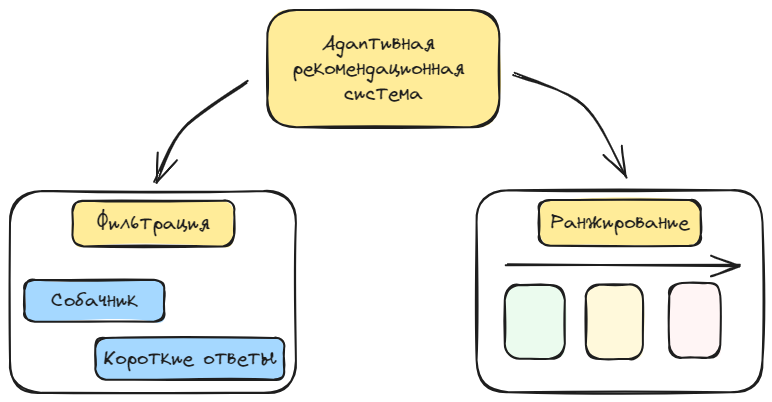
\includegraphics[width=0.5\textwidth]{assets/work/rating/bayes.excalidraw.png}
    \caption{Устройство байесового пересчета }
    \label{bayes}
\end{figure}

\textit{Лемма} Модель является игрой с нулевой суммой. 

\texit{Доказательство} Правило обновления


\textit{Лемма} Рейтинг Эло является устойчивым. В отсутствие изменений силы игрока в ходе обновлений рейтинга оценка станет истинной

\texit{Доказательство} Используем переход к модели Брэдлли-Терри.

Существуют также модель, учитывающие занятие одинаковой позиции в ступень ранга \cite{plackett1975analysis}\cite{luce2005individual}. 
Минус подходы заключается в вычислительной сложности пересчета.